\documentclass[12pt,a4paper]{article}
\usepackage[utf8]{inputenc}
\usepackage[spanish]{babel}
\usepackage[T1]{fontenc}
\usepackage{tocbibind} % Bibliografía en el indice
\usepackage{titlesec} % Posibilidad de editar los formatos de chapter
\usepackage{amsmath,amssymb,mathrsfs} % Matemáticas varias
\usepackage{tabularx} % Para las tablas
\usepackage[title]{appendix} % Para anexos
\usepackage[spanish]{babel} % Para modificar labels por defecto
\renewcommand{\baselinestretch}{1} % Interlineado. 1 es estandar
% --- Arreglos varios para la inclusion de imagenes
\usepackage{float}
\usepackage[pdftex]{graphicx}
\usepackage{subfigure}
\usepackage{graphicx}
\graphicspath{{T:/Tom/Facultad/Logos/}}
\usepackage[usenames,dvipsnames]{color}
\DeclareGraphicsExtensions{.png,.jpg,.pdf,.mps,.gif,.bmp}
% --- Para las dimensiones de los márgenes etc
\frenchspacing \addtolength{\hoffset}{-1.5cm}
\addtolength{\textwidth}{3cm} \addtolength{\voffset}{-2.5cm}
\addtolength{\textheight}{4cm}
% --- Para el encabezado
\setlength{\headheight}{33pt}
\usepackage{fancyhdr}
\fancyhead[R]{\includegraphics[height=1cm]{logo_fcefyn_nuevo.jpg}}\fancyhead[L]{\includegraphics[height=1cm]{unc1_a.jpg}}\fancyhead[C]{} \fancyfoot[C]{Página \thepage} \renewcommand{\footrulewidth}{0.4pt}
\pagestyle{fancy}
% --- Para las tablas
\usepackage{multirow} % Juntar filas
\newcolumntype{L}[1]{>{\raggedright\arraybackslash}p{#1}} % Justificar Izq
\newcolumntype{C}[1]{>{\centering\arraybackslash}p{#1}} % Justificar Centrar
\newcolumntype{R}[1]{>{\raggedleft\arraybackslash}p{#1}} % Justificar Der
\usepackage[numbered]{bookmark} % Para que figure las secciones en el PDF
\usepackage{listings} % Para poner código 
\usepackage{enumitem} % Para editar las propiedades de los items
\usepackage{color}
\usepackage[bottom]{footmisc} % Para las notas al pie de la página
\lstset{frame=single} % Código en un cuadro
\usepackage{tikz} % Para diagramas de estados en http://www.madebyevan.com/fsm/
% --- Para Anexo
\addto\captionsspanish{%
  \renewcommand\appendixname{ANEXO}
  \renewcommand\appendixpagename{ANEXOS}
}
% --- Para insertar codigo de Java
\usepackage{listings}
\usepackage{color}

\definecolor{dkgreen}{rgb}{0,0.6,0}
\definecolor{gray}{rgb}{0.5,0.5,0.5}
\definecolor{mauve}{rgb}{0.58,0,0.82}
\lstset{frame=tb,
  language=Java,
  aboveskip=3mm,
  belowskip=3mm,
  showstringspaces=false,
  columns=flexible,
  basicstyle={\small\ttfamily},
  numbers=none,
  numberstyle=\tiny\color{gray},
  keywordstyle=\color{blue},
  commentstyle=\color{dkgreen},
  stringstyle=\color{mauve},
  breaklines=true,
  breakatwhitespace=true,
  tabsize=3
}
% -------------------------------------------------------- %

\begin{document}

\begin{titlepage}
    \begin{center}
        \vspace*{1cm}
        
        \Large
        \textbf{Universidad Nacional de Córdoba\\
        		Facultad de Ciencias Exactas, Físicas y Naturales}
        
        \vspace{0.5cm}
        \includegraphics[width=0.5\textwidth]{logo_caratula.png}
        
        \vspace{1cm}
        
        \textbf{Trabajo Práctico Integrador}\\
        Programación Concurrente\\
        Docentes: \\
        Dr. Ing. Orlando Micolini\\
        Ing. Luis Orlando Ventre
        
        \vfill  
        
        \vspace{0.5cm}
        

        Alumnos:\\
        \Large
        Navarro, Sebastián\\
        
        \begin{large}
        \href{mailto:navarrosebastian95@gmail.com}{navarrosebastian95@gmail.com}\\
		\end{large} 
		
        Piñero, Tomás Santiago\\
        
        \begin{large}
        \href{mailto:tom-300@hotmail.com}{tom-300@hotmail.com}\\
		\end{large} 
		
        Año 2019\\
        
        
    \end{center}
\end{titlepage}
% -------------------------------------------------------- %
% --- Tabla de contenidos

\setcounter{secnumdepth}{3}
\setcounter{tocdepth}{5}
\tableofcontents

% -------------------------------------------------------- %

\newpage
\renewcommand{\baselinestretch}{1}
\setlength{\parskip}{0.5em}

\section{Enunciado}
\label{enunciado}

En este práctico se debe resolver el control de acceso a una playa de estacionamiento con 3 entradas (calles) diferentes. En esta playa hay 2 pisos, y en cada piso pueden estacionar 30 autos. La playa cuenta con 2 salidas diferentes y una única estación de pago (caja). En los accesos a la playa y en los egresos existen barreras que deben modelarse.

La playa cuenta con lugares (3) donde los vehículos se detienen cuando quieren entrar (barrera), una vez que ingresaron se les indica un piso y estacionan (puede ser piso 1 o piso 2). Se debe cuidar que no se permita el ingreso (superar barrera) a más vehículos de los espacios disponibles totales.

Los autos que se retiran de la playa deben liberar un espacio del piso en que se encontraban (diferenciar estacionamiento en cada piso). Cuando un vehículo se va a retirar puede optar por salida a calle 1 o salida a calle 2.
Luego debe abonar la estadía. El cobro de la estadía le lleva a un empleado promedio al menos 3 minutos. (Existe una sola caja)

En caso de que la playa esté llena, se debe encender un cartel luminoso externo que indica tal situación.

El sistema controlador debe estar conformado por distintos hilos, los cuales deben ser asignados a cada conjunto de responsabilidades afines en particular. Por ejemplo: Ingreso de vehículos, manejo de barreras, etcétera.

Debe realizar:
\begin{enumerate}
\item La red de Petri que modela el sistema.
\item Agregar las restricciones necesarias para evitar interbloqueos ni accesos cuando no hay lugar, mostrarlo con la herramienta elegida y justificarlo.
\item Simular la solución en un proyecto desarrollado con la herramienta adecuada (explique porque eligió la herramienta usada).
\item Colocar tiempo en las estación de pago caja (en la/s transición/es correspondiente/s).
\item Hacer la tabla de eventos.
\item Hacer la tabla de estados o actividades.
\item Determinar la cantidad de hilos necesarios (justificarlo)
\item Implementar dos casos de Políticas para:

\begin{itemize}
\item Prioridad llenar de vehículos planta baja (piso 1) y luego habilitar el piso superior. Prioridad salida indistinta (caja).
\item Prioridad llenado indistinta. Prioridad salida a calle 2.
\end{itemize}

\item Hacer el diagrama de clases.
\item Hacer los diagramas de secuencias.
\item Hacer el código.
\item Hacer el \emph{testing}.
\end{enumerate}

\section{Desarrollo}
\label{desarrollo}

\subsection{Requerimientos funcionales del sistema}
\begin{itemize}[leftmargin=1.5cm]
    \item El sistema no debe disparar transiciones no sensibilizadas.
    \item El sistema debe disparar transiciones sensibilizadas.
    \item El sistema debe conocer las transiciones sensibilizadas.
    \item El sistema debe tener la capacidad para disparar una transición sensibilizada por tiempo.
    \item El sistema no debe disparar una transición no sensibilizada por tiempo.
    \item El sistema debe tener prioridades/políticas de disparo entre transiciones.
    \item El sistema no debe permitir el acceso al monitor a más de un hilo.
\end{itemize}

\subsection{Tabla de estados}
\begin{table}[H]
\centering
\begin{tabular}[width=15cm]{ || C{1.5cm} | L{5cm} | L{8.5cm} || }
\hline
	Numero & Plaza & Estado  \\ \hline
	P0 & Limitador clientes calle 1 & Buffer que limita la cantidad de clientes a ingresar por la primer calle  \\ \hline
	P1 & Limitador clientes calle 2 & Buffer que limita la cantidad de clientes a ingresar por la segunda calle \\ \hline
	P2 & Limitador clientes calle 3 & Buffer que limita la cantidad de clientes a ingresar por la tercer calle  \\ \hline
	P3 & Autos esperando ingresar calle 1 & Cola de autos esperando para sacar el ticket en la primer calle  \\ \hline
	P4 & Autos esperando ingresar calle 2 & Cola de autos esperando para sacar el ticket en la segunda calle\\ \hline
	P5 & Autos esperando ingresar calle 3 & Cola de autos esperando para sacar el ticket en la tercer calle \\ \hline
	P6 & Auto pasando barrera 1 & El cliente sacó el ticket y la barrera se levanta  \\ \hline
	P7 & Auto pasando barrera 2 & El cliente sacó el ticket y la barrera se levanta   \\ \hline
	P8 & Auto pasando barrera 3 & El cliente sacó el ticket y la barrera se levanta  \\ \hline
	P9 & Barrera de calle 1 & Mutex para el uso de la barrera de la primer calle   \\ \hline
	P10 & Barrera de calle 2 & Mutex para el uso de la barrera de la segunda calle  \\ \hline
	P11 & Barrera de calle 3 & Mutex para el uso de la barrera de la tercer calle  \\ \hline
	P12 & Limitador de autos & Buffer que limita la cantidad de autos a utilizar la rampa  \\ \hline
	P13 & Autos por tomar rampa & Autos utilizando la rampa \\ \hline
	P14 & Auto buscando lugar arriba & Cliente buscando lugar para estacionar el auto en planta alta \\ \hline
	P15 & Auto buscando lugar abajo & Cliente buscando lugar para estacionar el auto en subsuelo \\ \hline
	P16 & Rampa & Mutex de uso de la rampa  \\ \hline
	P17 & Auto estacionado arriba & Auto estacionado en la planta de arriba  \\ \hline
	P18 & Auto estacionado abajo & Auto estacionado en el subsuelo  \\ \hline
	P19 & Lugares disponibles arriba & Cantidad de lugares disponibles en la planta alta \\ \hline
	P20 & Lugares disponibles abajo & Cantidad de lugares disponibles en el subsuelo  \\ \hline
	P21 & Cliente por bajar & Cliente sale de la planta alta y se dirije a la caja   \\ \hline
	P22 & Cliente por subir & Cliente sale del subsuelo y se dirije a la caja  \\ \hline
	P23 & Auto en rampa & Cliente esta bajando o subiendo por la rampa  \\ \hline
	P24 & Cliente por pagar & Cliente esperando para pagar el ticket  \\ \hline
	P25 & Cliente pagando & Cliente pagando el ticket \\ \hline
\end{tabular}
\end{table}
\begin{table}[H]
\centering
\begin{tabular}[width=15cm]{ || C{1.5cm} | L{5cm} | L{8.5cm} || }
\hline
	P26 & Cajero & Cajero \\ \hline
	P27 & Auto por salir & Auto por abonar el ticket \\ \hline
	P28 & Limitador de playa & Buffer que limita la cantidad de clientes que pueden dirigirse a la caja \\ \hline
	P29 & Cartel encendido & No hay mas lugar en la playa \\ \hline
	P30 & Cartel apagado & Hay lugar en la playa \\ \hline
\end{tabular}
\caption{Tabla de estados.}
\label{table:plazas}
\end{table}

\subsection{Tabla de eventos}
\begin{table}[H]
\centering
\begin{tabular}[width=15cm]{ || C{1.5cm} | L{5cm} | L{8.5cm} || }
\hline
	Numero & Plaza & Estado  \\ \hline
	T0 & Entrar calle 1 & Autos ingresando por la primer calle  \\ \hline
	T1 & Entrar calle 2 & Autos ingresando por la segunda calle \\ \hline
	T2 & Entrar calle 3 & Autos ingresando por la tercer calle \\ \hline
	T3 & Sacar ticket 1 & El cliente saca el ticket para levantar la barrera  \\ \hline
	v4 & Sacar ticket 2 & El cliente saca el ticket para levantar la barrera \\ \hline
	T5 & Sacar ticket 3 3 & El cliente saca el ticket para levantar la barrera \\ \hline
	T6 & Levantar barrera 1 & Una vez sacado el ticket, se levanta la barrera para el ingreso a la playa  \\ \hline
	T7 & Levantar barrera 2 & Una vez sacado el ticket, se levanta la barrera para el ingreso a la playa   \\ \hline
	T8 & Levantar barrera 3 & Una vez sacado el ticket, se levanta la barrera para el ingreso a la playa  \\ \hline
	T9 & Subir por rampa & El cliente sube a la planta alta del estacionamiento   \\ \hline
	T10 & Bajar por rampa & El cliente va a la planta baja del estacionamiento  \\ \hline
	T11 & Buscar lugar arriba & El cliente busca lugar para estacionar en la planta alta  \\ \hline
	T12 & Buscar lugar abajo & El cliente busca lugar para estacionar en la planta baja  \\ \hline
	T13 & Aguardar salida arriba & El cliente dejó el auto estacionado en la planta alta \\ \hline
	T14 & Aguardar salida abajo & El cliente dejó el auto estacionado en la planta baja \\ \hline
	T15 & Bajar & El cliente de la planta alta se dirige a la salida \\ \hline
	T16 & Subir & El cliente de la planta baja se dirige a la salida  \\ \hline
	T17 & Esperar caja & El cliente se dirige a la caja  \\ \hline
	T18 & Pagar & El cliente paga el ticket en la caja  \\ \hline
	T19 & Devolver cajero & El cliente elige la salida \\ \hline
	T20 & Salir por calle 1 & El cliente sale por la calle 1  \\ \hline
	T21 & Salir por calle 2 & El cliente sale por la calle 2   \\ \hline
	T22 & Encender el cartel 2 & Se llenó la playa, se enciende el cartel   \\ \hline
	T23 & Apagar cartel 2 & Hay lugar en la playa, se apaga el cartel   \\ \hline
\end{tabular}
\caption{Tabla de eventos.}
\label{table:transiciones}
\end{table}

\subsection{Hilos}
 Los hilos son aquellos que realizan un conjunto de acciones, por lo que para determinar la cantidad de hilos necesarios, se realizó una modularización de la red en actividades, por lo tanto, la cantidad de hilos utilizados son 9:

\begin{enumerate}[leftmargin=1.5cm]
\item Entrada calle 1: T0 -- T3.
\item Entrada calle 2: T1 -- T4.
\item Entrada calle 3: T2 -- T5.
\item Acceder a la playa: T6 -- T7 -- T8.
\item Planta Alta: T9 -- T11 -- T13 -- T15.
\item Planta Baja: T10 -- T12 -- T14 -- T16.
\item Cobrar tickets: T17 -- T18 -- T19.
\item Salida: T20 -- T21.
\item Cartel: T22 -- T23.
\end{enumerate}

\subsubsection*{Hilos 1, 2 y 3}
Los 3 hilos iniciales en las entradas son de existencia trivial, donde cada calle (o entrada) es independiente una de la otra, y cada una cuenta con sus propios recursos. Estos hilos representan a los autos pasando las barreras.
\subsubsection*{Hilo 4}
La segunda etapa de la red, el tramo que abarca el acceso a la playa.
Este hilo resulta indispensable para la fluidez de la red. Al ser un conjunto de transiciones de mucha demanda, resulta necesario contar con un hilo que tenga la mayor parte del tiempo alguna de sus transiciones sensibilizadas, de modo que éste se encole la menor cantidad de veces posible y en consecuencia, los alrededores de la red no conduzcan a un interbloqueo.
\subsubsection*{Hilos 5, 6 y 7}
Se independizan esos 3 conjuntos de transiciones de la red para modularizarla lo más posible y así elevar su concurrencia, por lo que se asigna un hilo a cada piso (hilos 5 y 6, respectivamente) y otro que maneja la caja (hilo 7). Además, esta distribución conserva la linealidad de la red cuando se la compara con la realidad, resulta intuitivo pensar que la linea de Planta Alta, Planta Baja y Caja es administrado de manera completa por un hilo cada una.
\subsubsection*{Hilo 8}
Se asigna un hilo a la dupla de transiciones T20 y T21 para resolver el último conflicto de la red, de modo que se puede implementar más fácilmente una política que las administre, y que además asegure un comportamiento consistente. 
\subsubsection*{Hilo 9}
Se encarga del manejo del cartel de la playa.

\subsubsection*{Discusiones}
Al comienzo se había implementado una política \emph{FIFO} para el orden de disparo de cada hilo con el fin de verificar que el monitor implementado funcionara correctamente. Esto causó que si el hilo que ingresó al monitor no podía disparar el primero de los disparos listado en el archivo de texto asignado, se encolaba allí dentro esperando poder disparar dicha transición. Este diseño trajo serios problemas de interbloqueo, ya que la política le indicaba al hilo que dispare la primer transición asignada, independientemente si estaba sensibilizada o no, por lo que si la transición no estaba sensibilizada no permitía la evolución de la red.

Esto fue solucionado implementando dentro de la clase Políticas, un método de consulta, donde el hilo le consulta cuáles de sus transiciones puede dispararse en ese momento, proporcionándole la información mas óptima para la fluidez de la red. De este diseño se habla con mayor detalle en la \textit{sección 2.5}.  

Una vez solucionado el problema de las políticas, se probó la distribución de los hilos de 3 formas diferentes, añadiendo variantes en el conjunto de transiciones T6 -- T7 -- T8 -- T9 -- T10, que es la sección de la red que traslada los autos de la entrada a sus respectivos estacionamientos.

Finalmente resultó irrelevante el modo en que estas se distribuían, ya que ninguna afectaba el rendimiento ni ofrecía alguna mejora, pero se optó por la distribución descripta al comienzo de la sección, para conservar la linealidad de los hilos con respecto a sus tareas en la red.

\subsection{Parámetros del Sistema}
El proyecto esta diseñado para parametrizarse a través de archivos de texto plano. 

\begin{itemize}[leftmargin=1.5cm]
    \item hilos.txt -- se carga un hilo por fila. Cada valor de la fila corresponde a la \emph{ID} de la transición.
    \item incidencia\_mas.txt -- contiene la matriz de incidencia positiva generada por PIPE.
    \item incidencia\_menos.txt -- contiene la matriz de incidencia negativa generada por PIPE, pero modificada para que contenga un valor negativo en vez de positivo.
    \item inhibidas.txt -- es la matriz de inhibición generada por el PIPE.
    \item intervalos.txt -- incluye la matriz de intervalos temporales de las transiciones de la red.
    \item marcado.txt -- incluye el marcado inicial de la red.
    \item pInvariantes.txt -- conserva el formato generado por PIPE, pero se eliminan todos los dígitos no numéricos, de modo que el ultimo valor de cada fila es el resultado de la suma de cada una de las plazas anteriores. Cada salto de linea es un P-Invariante diferente.
    \item tInvariantes.txt -- al igual que con las P-Invariantes, se eliminan todos los identificadores de las transiciones mientras se conserva el mismo formato original generado por PIPE.
\end{itemize}

Una vez realizados los disparos, el sistema genera el archivo `output.txt' en el cual se encuentra la secuencia de disparos realizada.

\subsection{Red de Petri}
Al tratarse de una red que está acotada, se tiene una secuencia de disparos infinita, por lo tanto la red es monótona.

\textbf{Semántica utilizada para las transiciones temporizadas}

Se tomo la primera de las semánticas especificadas en \textit{“Redes de Petri Temporales 2017.pdf” -- Hoja 11}, por lo tanto el disparo se realiza en dos etapas:

\begin{itemize}[leftmargin=1.5cm]
    \item Transcurre un determinado tiempo desde que una transición se sensibiliza.
    \item Se retiran y colocan las marcas de forma atómica.
\end{itemize}

Cabe mencionar que esto se usa para ambos tipos de transiciones: inmediatas y temporales, ya que en el caso de la inmediata, el paso 1 implica un intervalo de tiempo nulo.

Al tener un arco lector, no se utiliza la matriz de incidencia combinada para realizar el cálculo del estado siguiente de la red, ya que este tipo de arco puede definirse como un arco común que entra y sale de una misma transición, por lo que se verá reflejado como un 0 en la matriz de incidencia combinada. Debido a esto se realiza el cálculo del estado siguiente en dos etapas: primero se realiza la toma de tokens utilizando la matriz de incidencia negativa y luego se realiza la inserción de tokens utilizando la matriz de incidencia positiva.

\subsubsection{Tiempos}
Para las transiciones temporizadas se utiliza una clase dedicada a ``cronometrarlas”: ‘Tiempos’. Una transición con tiempo se ``cronometra” desde el inicio de su sensibilización, y en el momento en el que se la quiere disparar, se debe verificar que el tiempo dicho esté dentro de su intervalo de tiempo $[a_i , b_i]$. Si el disparo se quiere realizar antes del límite inferior $(a_i)$, el hilo debe dormir $a_i-x$ segundos, donde $x$ es el tiempo transcurrido desde que se sensibilizó la transición.

Los tiempos se asignan a cada transición desde el archivo \textit{`intervalos.txt'}. Éste cuenta con 2 columnas por transición, donde la primera indica el \textit{$a_i$} (alfa) y la segunda el \textit{$b_i$} (beta). 

Una transición no temporizada o inmediata se parametriza con $a_i = 0 $ y $b_i = 0$. En el caso de esta red en particular \textit{T13, T14} y \textit{T18} representan a los tiempos del estacionamiento y cajero respectivamente, a los cuales se les asignó los siguientes valores, expresados en el orden de los \textit{milisegundos}.

\begin{itemize}[leftmargin=1.5cm]
    \item T13 -- [200, 1500]
    \item T14 -- [150, 1800]
    \item T18 -- [10, 300]
\end{itemize}

Resulta importante la asignación de estos tiempos. Un alfa muy próximo a 0 es rápidamente sensibilizada, pero si es acompañada de un beta cercano, la ventana de disparo de la transición será excedido con mucha certeza, y en consecuencia pocas veces o incluso nunca será disparada, acarreando problemas de fluidez y un eventual interbloqueo.

Debido al orden de magnitud de tiempo, es importante ajustar estos valores acorde al poder de procesamiento de cada computador. El lapso de tiempo entre la lectura de una linea y otra pasa a ser relevante cuando se manejan dichas magnitudes.

\begin{figure}[H]
    \centering
    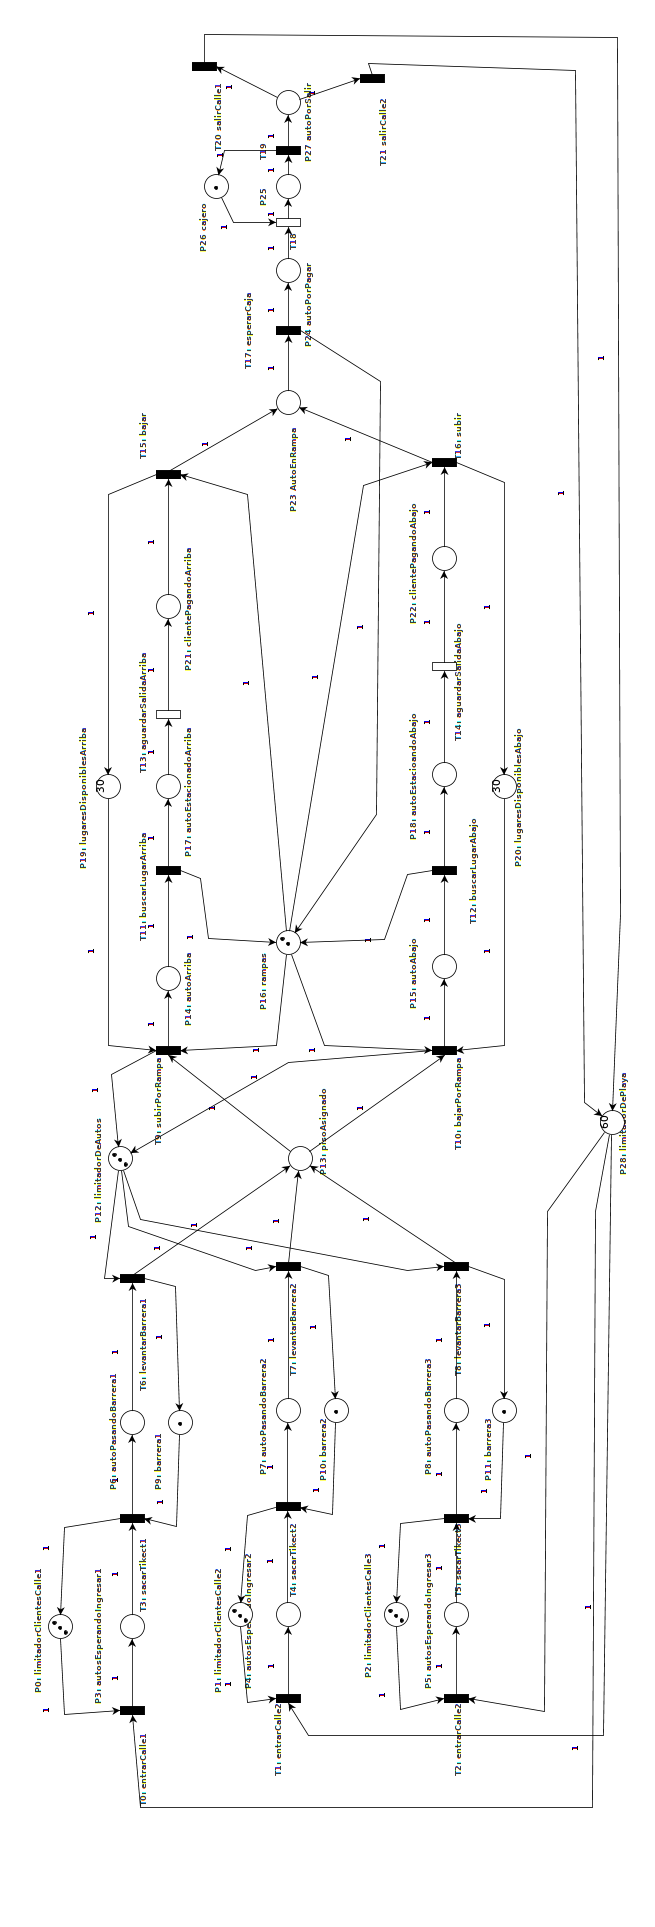
\includegraphics[scale=0.4]{estacionamiento_2019}
    \label{fig:rdp}
    \caption{Red de Petri que modela el sistema.}
\end{figure}

\subsection{Políticas}
Aquel conjunto de transiciones pertenecientes a un hilo en particular, que no requieran el tratado de políticas específicas, se dispararan preferentemente en el orden dispuesto en el archivo de texto `hilos.txt', siendo este un posible orden de prioridades, para garantizar el orden y la fluidez de la red. Ejemplificando, suponga un hilo que haya conseguido acceso al monitor y que lleva parametrizadas \textit{[T0    T3    T6]}; la transición \textit{T0} será la primera en ser evaluada en función de su estado de sensibilizada, de poder dispararse, se procede, caso contrario, se intentará con T3. Si finalmente, ninguna de las 3 transiciones del hilo puede ser disparada en ese instante, éste se encolará dentro del monitor con el primer parámetro de la lista, en este caso \textit{T0}.

Por otro lado, las transiciones que requieren tratado de políticas especificas, son administradas por la clase `Politicas' del proyecto y obedecen al enunciado.

Cabe mencionar que se interpretó por `prioridad' a un piso o una salida como la opción más probable que puede llegar a suceder, por lo que para la primer política, el 70\% de los autos irá a planta baja, mientras que el 30\% restante irá a planta alta. Estos mismos porcentajes se utilizan en la segunda política para la elección de la calle de salida (70\% para la salida 2 y 30\% para la salida 1).

La elección de esta política se realiza por medio del constructor de la clase `Politicas', donde se pasa como parámetro el número de política que se desea utilizar: 1 para la primer política ó 2 para la segunda.

\subsection{Análisis de Invariantes}
El análisis de invariantes es utilizado para la realización del \emph{testing} del código. Para que éste sea exitoso ambos invariantes (de plaza y transiciones) deben cumplirse, ya que el hecho de que no se cumpla alguno implica que el sistema está funcionando de manera incorrecta. Si no se cumplen los invariantes de plaza significa que no se está respetando la cantidad de recursos existentes en la red, mientras que si no se cumplen los invariantes de transiciones se verifica que los bucles posibles que posee la red no se están realizando, por lo que los disparos están ocurriendo en manera incorrecta. 

\subsubsection{P-Invariantes}
Un invariante P indica que el número de tokens en todas las marcas alcanzables satisface una invariante lineal.
Un invariante algebraico es una cierta combinación de las componentes de una matriz cuyo valor numérico no queda alterado al hacer un cambio de base.
Las invariantes la red generadas por PIPE son las siguientes:

\begin{enumerate}[leftmargin=1.5cm]
\item Limitador de autos en la primer entrada.

        \verb|M(P0) + M(P3) = 3|
        
\item Limitador de autos en la segunda entrada.

        \verb|M(P1) + M(P4) = 3 |

\newpage
\item Limitador de autos en la tercer entrada.

        \verb|M(P2) + M(P5) = 3 |

\item Barrera de la primer entrada.

        \verb|M(P6) + M(P9) = 1|
        
\item Barrera de la segunda entrada.

        \verb|M(P10) + M(P7) = 1 |
        
\item Barrera de la tercer entrada.

        \verb|M(P11) + M(P8) = 1 |

\item Regulador de autos para acceso a la rampa.

        \verb|M(P12) + M(P13) = 3 |

\item Limitador de autos en planta alta.

        \verb|M(P14) + M(P17) + M(P19) + M(P21) = 30 |

\item Limitador de autos en planta baja.

        \verb|M(P15) + M(P18) + M(P20) + M(P22) = 30 |

\item Regulador de autos para acceso y egreso a las plantas de la playa.

        \verb|M(P14) + M(P15) + M(P16) + M(P23) = 2 |

\item Regulador de autos en cola para pagar.

        \verb|M(P21) + M(P22) + M(P23) + M(P24) + M(P31) = 3|
        
\item Empleado de caja.

        \verb|10- M(P25) + M(P26) = 1 |     
        
\item Cartel de la playa.        

        \verb|M(P29) + M(P30) = 1|
        
\item Limitador de clientes totales que pueden encontrarse en el sistema.

        \verb|M(P13) + M(P14) + M(P15) + M(P17) + M(P18) + M(P21) + M(P22) + M(P23) |
        
        \verb|+ M(P24) + M(P25) + M(P27) + M(P28) + M(P3) + M(P4) + M(P5) + M(P6) |
        
        \verb|+ M(P7) + M(P8) = 60|   
\end{enumerate}

Luego de un disparo, y en consecuencia, luego de cada evolución de la red, se evalúa cada una de las 14 condiciones de P-Invariantes arriba listadas. 
Una bandera booleana inicializada en \textit{true} permanece en ese estado siempre que el resultado del análisis sea satisfactorio, pero en caso de haber una inconsistencia en la red que viole el análisis, la bandera pasará al estado \textit{false} y permanecerá en ese estado hasta el fin de la ejecución, indicando que como mínimo una P-Invariante no se cumplió.

\subsubsection{T-Invariantes}
Estas indican posibles bucles (\emph{loops}) en la red. Es decir, una secuencia de disparos que tenga asociado un invariante de transición, vuelve al mismo marcado desde el que partió.

\begin{enumerate}[leftmargin=1.5cm]
    \item Entra por la primer calle, estaciona en planta alta, y sale por calle 1.
    
    \verb|[T0, T3, T6, T9, T11, T13, T15, T17, T18, T19, T20]|
    
    \item Entra por la primer calle, estaciona en planta alta, y sale por calle 2.
    
    \verb|[T0, T3, T6, T9, T11, T13, T15, T17, T18, T19, T21]|
    
    \item Entra por la primer calle, estaciona en planta baja, y sale por calle 1.
    
    \verb|[T0, T3, T6, T10, T12, T14, T16, T17, T18, T19, T20]|
    
    \item Entra por la primer calle, estaciona en planta baja, y sale por calle 2.
    
    \verb|[T0, T3, T6, T10, T12, T14, T16, T17, T18, T19, T21]|
    
    \item Entra por la segunda calle, estaciona en planta alta, y sale por calle 1.
    
    \verb|[T1, T4, T7, T9, T11, T13, T15, T17, T18, T19, T20]|
    
    \item Entra por la segunda calle, estaciona en planta alta, y sale por calle 2.
    
    \verb|[T1, T4, T7, T9, T11, T13, T15, T17, T18, T19, T21]|
    
    \item Entra por la segunda calle, estaciona en planta baja, y sale por calle 1.
    
    \verb|[T1, T4, T7, T10, T12, T14, T16, T17, T18, T19, T20]|
    
    \item Entra por la segunda calle, estaciona en planta baja, y sale por calle 2.
    
    \verb|[T1, T4, T7, T10, T12, T14, T16, T17, T18, T19, T21]|
    
    \item Entra por la tercer calle, estaciona en planta alta, y sale por calle 1.
    
    \verb|[T2, T5, T8, T9, T11, T13, T15, T17, T18, T19, T20]|
    
    \item Entra por la tercer calle, estaciona en planta alta, y sale por calle 2.
    
    \verb|[T2, T5, T8, T9, T11, T13, T15, T17, T18, T19, T21]|
    
    \item Entra por la tercer calle, estaciona en planta baja, y sale por calle 1.
    
    \verb|[T2, T5, T8, T10, T12, T14, T16, T17, T18, T19, T20]|
    
    \item Entra por la tercer calle, estaciona en planta baja, y sale por calle 2.
    
    \verb|[T2, T5, T8, T10, T12, T14, T16, T17, T18, T19, T21]|
    
    \item Encender y apagar el cartel.
    
    \verb|[T22, T23]|
\end{enumerate}

Se almacena en un arreglo la secuencia de disparos durante la ejecución, para luego hacer uso de las T-Invariantes y verificar que se cumplen los ciclos de disparos de la red. 

En el caso ideal, si la ejecución finalizase en el mismo estado de transiciones sensibilizadas que al inicio de la ejecución (es decir, todos los ciclos de T-Invariante son completados), la intersección entre el conjunto total de disparos y cada vector de secuencia (completo) de T-Invariante arriba listado, resultaría en un remanente de 0 disparos, lo cual indicaría un perfecto funcionamiento de la red.

No obstante, como la ejecución tiene una cantidad de disparos predefinida, dicha intersección dejará remanentes de disparos que no han llegado a completar su ciclo, pero esto no implica una inconsistencia en la red o en el monitor, ya que al estar limitada en cantidad de disparos, dichos remanentes serán secuencias parciales de los invariantes.

\subsubsection{Maquina de Estados de la Red}
\begin{center}
\begin{tikzpicture}[scale=0.2]
\tikzstyle{every node}+=[inner sep=0pt]
\draw [black] (3.2,-30.5) circle (3);
\draw (3.2,-30.5) node {$E_0$};
\draw [black] (7.8,-7.4) circle (3);
\draw (7.8,-7.4) node {$E_{11}$};
\draw [black] (16.7,-6.8) circle (3);
\draw (16.7,-6.8) node {$E_{21}$};
\draw [black] (26.1,-6.8) circle (3);
\draw (26.1,-6.8) node {$E_{31}$};
\draw [black] (40.9,-10.1) circle (3);
\draw (40.9,-10.1) node {$E_{41}$};
\draw [black] (48.3,-10.1) circle (3);
\draw (48.3,-10.1) node {$E_{51}$};
\draw [black] (55.9,-10.1) circle (3);
\draw (55.9,-10.1) node {$E_{61}$};
\draw [black] (64.6,-10.1) circle (3);
\draw (64.6,-10.1) node {$E_{71}$};
\draw [black] (71.9,-19) circle (3);
\draw (71.9,-19) node {$E_{1}$};
\draw [black] (72.9,-34.5) circle (3);
\draw (72.9,-34.5) node {$E_{2}$};
\draw [black] (45.4,-50.5) circle (3);
\draw (45.4,-50.5) node {$E_{Fin}$};
\draw [black] (45.4,-50.5) circle (2.4);
\draw [black] (72.9,-48.4) circle (3);
\draw (72.9,-48.4) node {$E_{3}$};
\draw [black] (37.9,-31.6) circle (3);
\draw (37.9,-31.6) node {$E_{42}$};
\draw [black] (46.4,-31.6) circle (3);
\draw (46.4,-31.6) node {$E_{52}$};
\draw [black] (54.2,-31.6) circle (3);
\draw (54.2,-31.6) node {$E_{62}$};
\draw [black] (63.1,-28.4) circle (3);
\draw (63.1,-28.4) node {$E_{72}$};
\draw [black] (7.8,-20.8) circle (3);
\draw (7.8,-20.8) node {$E_{12}$};
\draw [black] (17.5,-20.8) circle (3);
\draw (17.5,-20.8) node {$E_{22}$};
\draw [black] (27.1,-20.8) circle (3);
\draw (27.1,-20.8) node {$E_{32}$};
\draw [black] (10.6,-40.5) circle (3);
\draw (10.6,-40.5) node {$E_{13}$};
\draw [black] (18.9,-40.5) circle (3);
\draw (18.9,-40.5) node {$E_{23}$};
\draw [black] (28.5,-40.5) circle (3);
\draw (28.5,-40.5) node {$E_{33}$};
\draw [black] (12.6,-52.4) circle (3);
\draw (12.6,-52.4) node {$E_{4}$};
\draw [black] (2.249,-27.657) arc (-165.56397:-216.96048:21.158);
\fill [black] (5.83,-9.66) -- (4.95,-10) -- (5.75,-10.6);
\draw (1.25,-17.94) node [left] {$0$};
\draw [black] (9.918,-5.331) arc (118.25228:69.46132:5.345);
\fill [black] (14.32,-5.03) -- (13.75,-4.29) -- (13.4,-5.22);
\draw (11.98,-4.14) node [above] {$3$};
\draw [black] (18.942,-4.859) arc (115.71917:64.28083:5.665);
\fill [black] (23.86,-4.86) -- (23.35,-4.06) -- (22.92,-4.96);
\draw (21.4,-3.8) node [above] {$6$};
\draw [black] (28.969,-5.945) arc (99.96617:54.89425:12.962);
\fill [black] (38.67,-8.11) -- (38.3,-7.24) -- (37.72,-8.06);
\draw (34.77,-5.47) node [above] {$9$};
\draw [black] (42.041,-7.414) arc (-226.25198:-313.74802:3.7);
\fill [black] (47.16,-7.41) -- (46.93,-6.5) -- (46.23,-7.22);
\draw (44.6,-5.89) node [above] {$11$};
\draw [black] (49.417,-7.399) arc (-225.0872:-314.9128:3.8);
\fill [black] (54.78,-7.4) -- (54.57,-6.48) -- (53.86,-7.19);
\draw (52.1,-5.79) node [above] {$13$};
\draw [black] (57.445,-7.594) arc (129.04587:50.95413:4.453);
\fill [black] (63.06,-7.59) -- (62.75,-6.7) -- (62.12,-7.48);
\draw (60.25,-6.1) node [above] {$15$};
\draw [black] (67.321,-11.337) arc (57.05969:21.65921:10.109);
\fill [black] (71.22,-16.09) -- (71.39,-15.16) -- (70.46,-15.53);
\draw (70.2,-11.98) node [right] {$17$};
\draw [black] (73.933,-21.192) arc (34.71237:-27.3296:10.57);
\fill [black] (74.63,-32.06) -- (75.45,-31.58) -- (74.56,-31.12);
\draw (76.39,-26.49) node [right] {$18$};
\draw [black] (74.711,-36.876) arc (28.38342:-28.38342:9.621);
\fill [black] (74.71,-46.02) -- (75.53,-45.56) -- (74.65,-45.08);
\draw (76.37,-41.45) node [right] {$19$};
\draw [black] (3.329,-27.513) arc (-190.76078:-219.98234:10.362);
\fill [black] (5.57,-22.79) -- (4.67,-23.08) -- (5.44,-23.72);
\draw (3.44,-23.95) node [left] {$1$};
\draw [black] (10.333,-19.237) arc (109.37089:70.62911:6.984);
\fill [black] (14.97,-19.24) -- (14.38,-18.5) -- (14.05,-19.44);
\draw (12.65,-18.34) node [above] {$4$};
\draw [black] (20.051,-19.266) arc (108.73721:71.26279:7);
\fill [black] (24.55,-19.27) -- (23.95,-18.54) -- (23.63,-19.48);
\draw (22.3,-18.4) node [above] {$7$};
\draw [black] (28.861,-18.373) arc (140.74984:114.82746:26.094);
\fill [black] (38.11,-11.2) -- (37.17,-11.08) -- (37.59,-11.99);
\draw (31.92,-13.77) node [above] {$9$};
\draw [black] (35.335,-30.048) arc (-124.49606:-145.50394:25.92);
\fill [black] (35.33,-30.05) -- (34.96,-29.18) -- (34.39,-30.01);
\draw (29.86,-27.49) node [below] {$10$};
\draw [black] (27.39,-9.51) -- (36.61,-28.89);
\fill [black] (36.61,-28.89) -- (36.72,-27.95) -- (35.82,-28.38);
\draw (32.71,-18.14) node [right] {$10$};
\draw [black] (44.727,-34.02) arc (-54.18109:-125.81891:4.403);
\fill [black] (44.73,-34.02) -- (43.79,-34.08) -- (44.37,-34.89);
\draw (42.15,-35.35) node [below] {$12$};
\draw [black] (52.227,-33.775) arc (-62.68448:-117.31552:4.199);
\fill [black] (52.23,-33.77) -- (51.29,-33.7) -- (51.75,-34.59);
\draw (50.3,-34.74) node [below] {$14$};
\draw [black] (61.092,-30.601) arc (-53.90746:-86.54039:7.454);
\fill [black] (61.09,-30.6) -- (60.15,-30.67) -- (60.74,-31.48);
\draw (60.88,-32.14) node [below] {$16$};
\draw [black] (70.328,-21.553) arc (-35.05663:-51.167:24.978);
\fill [black] (70.33,-21.55) -- (69.46,-21.92) -- (70.28,-22.5);
\draw (68.65,-25.74) node [right] {$17$};
\draw [black] (70.221,-49.748) arc (-65.92694:-105.33938:32.67);
\fill [black] (48.25,-51.43) -- (48.89,-52.12) -- (49.16,-51.15);
\draw (59.84,-53.26) node [below] {$20+21$};
\draw [black] (7.756,-39.595) arc (-117.55285:-169.44427:8.686);
\fill [black] (7.76,-39.59) -- (7.28,-38.78) -- (6.81,-39.67);
\draw (4.21,-38.45) node [left] {$2$};
\draw [black] (13.26,-39.172) arc (103.28162:76.71838:6.485);
\fill [black] (16.24,-39.17) -- (15.58,-38.5) -- (15.35,-39.47);
\draw (14.75,-38.5) node [above] {$5$};
\draw [black] (21.497,-39.04) arc (107.57316:72.42684:7.298);
\fill [black] (25.9,-39.04) -- (25.29,-38.32) -- (24.99,-39.28);
\draw (23.7,-38.2) node [above] {$8$};
\draw [black] (36.835,-34.396) arc (-28.06613:-65.06401:11.903);
\fill [black] (36.84,-34.4) -- (36.02,-34.87) -- (36.9,-35.34);
\draw (36.33,-37.92) node [below] {$10$};
\draw [black] (29.249,-37.595) arc (164.77394:150.84548:110.873);
\fill [black] (39.4,-12.7) -- (38.58,-13.15) -- (39.45,-13.64);
\draw (32.83,-23.93) node [left] {$9$};
\draw [black] (9.892,-51.12) arc (-120.55379:-192.98589:16.369);
\fill [black] (9.89,-51.12) -- (9.46,-50.28) -- (8.95,-51.14);
\draw (2.44,-44.44) node [left] {$22$};
\draw [black] (42.564,-51.477) arc (-72.5338:-100.83569:55.383);
\fill [black] (42.56,-51.48) -- (41.65,-51.24) -- (41.95,-52.19);
\draw (29.27,-54.54) node [below] {$23$};
\draw [black] (6.117,-29.85) arc (130.29544:-157.70456:2.25);
\draw (10.52,-32.54) node [right] {$\overline{0}+\overline{1}+\overline{2}+\overline{22}$};
\fill [black] (5.49,-32.42) -- (5.63,-33.35) -- (6.39,-32.71);
\draw [black] (4.93,-6.567) arc (281.54126:-6.45874:2.25);
\draw (2.28,-1.38) node [left] {$\overline{3}$};
\fill [black] (6.72,-4.62) -- (7.05,-3.73) -- (6.07,-3.93);
\draw [black] (12.981,-42.305) arc (80.56505:-207.43495:2.25);
\draw (15.15,-47.04) node [below] {$\overline{5}$};
\fill [black] (10.62,-43.49) -- (9.99,-44.2) -- (10.98,-44.36);
\draw [black] (21.366,-42.187) arc (83.35775:-204.64225:2.25);
\draw (23.75,-46.89) node [below] {$\overline{8}$};
\fill [black] (19.06,-43.48) -- (18.47,-44.22) -- (19.47,-44.34);
\draw [black] (30.864,-42.328) arc (80.02604:-207.97396:2.25);
\draw (33.64,-47.08) node [below] {$\overline{10}$};
\fill [black] (28.49,-43.49) -- (27.86,-44.19) -- (28.84,-44.36);
\draw [black] (11.129,-55.001) arc (-1.76672:-289.76672:2.25);
\draw (6.42,-57.54) node [left] {$\overline{23}$};
\fill [black] (9.64,-52.81) -- (8.86,-52.29) -- (8.83,-53.29);
\draw [black] (69.925,-48.121) arc (292.37935:4.37935:2.25);
\draw (66.52,-43.58) node [left] {$\overline{20}+\overline{21}$};
\fill [black] (71.31,-45.87) -- (71.47,-44.94) -- (70.54,-45.32);
\draw [black] (71.173,-36.939) arc (-7.56336:-295.56336:2.25);
\draw (66.29,-38.89) node [left] {$\overline{19}$};
\fill [black] (69.91,-34.61) -- (69.19,-34.01) -- (69.05,-35);
\draw [black] (10.377,-22.314) arc (87.30053:-200.69947:2.25);
\draw (13.06,-26.94) node [below] {$\overline{4}$};
\fill [black] (8.17,-23.77) -- (7.63,-24.54) -- (8.63,-24.59);
\draw [black] (19.493,-23.027) arc (69.56239:-218.43761:2.25);
\draw (20.54,-27.89) node [below] {$\overline{7}$};
\fill [black] (16.94,-23.74) -- (16.2,-24.31) -- (17.13,-24.66);
\draw [black] (27.898,-23.68) arc (43.22627:-244.77373:2.25);
\draw (24.68,-28.13) node [below] {$\overline{10}$};
\fill [black] (25.3,-23.19) -- (24.37,-23.37) -- (25.06,-24.1);
\draw [black] (15.889,-9.676) arc (11.99467:-276.00533:2.25);
\draw (10.62,-12.3) node [below] {$\overline{6}$};
\fill [black] (13.92,-7.91) -- (13.04,-7.58) -- (13.25,-8.56);
\draw [black] (25.364,-9.696) arc (13.48154:-274.51846:2.25);
\draw (20.15,-12.42) node [below] {$\overline{9}$};
\fill [black] (23.35,-7.98) -- (22.46,-7.68) -- (22.69,-8.65);
\draw [black] (37.919,-28.612) arc (207.36933:-80.63067:2.25);
\draw (43.11,-25.06) node [above] {$\overline{12}$};
\fill [black] (40.28,-29.8) -- (41.22,-29.87) -- (40.76,-28.99);
\draw [black] (46.246,-28.616) arc (210.68227:-77.31773:2.25);
\draw (51.21,-24.87) node [above] {$\overline{14}$};
\fill [black] (48.68,-29.66) -- (49.62,-29.68) -- (49.11,-28.82);
\draw [black] (53.945,-28.623) arc (212.61878:-75.38122:2.25);
\draw (58.75,-24.77) node [above] {$\overline{16}$};
\fill [black] (56.41,-29.59) -- (57.35,-29.58) -- (56.81,-28.73);
\draw [black] (62.322,-25.515) arc (222.83233:-65.16767:2.25);
\draw (65.62,-21.08) node [above] {$\overline{17}$};
\fill [black] (64.92,-26.03) -- (65.84,-25.85) -- (65.16,-25.12);
\draw [black] (43.232,-11.968) arc (79.03378:-208.96622:2.25);
\draw (45.92,-16.73) node [below] {$\overline{11}$};
\fill [black] (40.84,-13.09) -- (40.19,-13.78) -- (41.17,-13.97);
\draw [black] (50.548,-12.069) arc (76.517:-211.483:2.25);
\draw (53.01,-16.87) node [below] {$\overline{13}$};
\fill [black] (48.1,-13.08) -- (47.43,-13.74) -- (48.4,-13.98);
\draw [black] (58.167,-12.046) arc (77.08915:-210.91085:2.25);
\draw (60.68,-16.84) node [below] {$\overline{15}$};
\fill [black] (55.73,-13.08) -- (55.07,-13.75) -- (56.04,-13.98);
\draw [black] (65.144,-7.162) arc (197.24515:-90.75485:2.25);
\draw (70.84,-4.19) node [above] {$\overline{17}$};
\fill [black] (67.26,-8.74) -- (68.18,-8.98) -- (67.88,-8.03);
\draw [black] (72.641,-16.105) arc (193.37843:-94.62157:2.25);
\draw (78.5,-13.39) node [above] {$\overline{18}$};
\fill [black] (74.65,-17.83) -- (75.54,-18.13) -- (75.31,-17.16);
\end{tikzpicture}
\end{center}

Este autómata finito parte de las T-Invariantes de la red descriptas en la \textit{subsección} anterior, que añade mayor simplicidad a la hora de reconocer los ciclos que puede realizar la Red.

A grandes rasgos, pueden identificarse los 3 conjuntos de entradas al estacionamiento, ambas plantas, el cajero y las instancias de salida a la calle. Y además se visualiza el corto ciclo que recorre el autómata para encender el cartel.

Esta maquina de estados finito fue implementada utilizando una clase de tipo \textit{Enum}, la cual tiene 23 enumeraciones (i.e. cantidad de estados), cada una con un método que recibe el valor de la variable como parámetro, y devuelve al llamado el próximo estado (Enum) en caso de cumplir con la secuencia del autómata, de modo que evoluciona hasta eventualmente llegar al estado \textit{EFin}.

Resulta una herramienta muy útil a la hora de verificar las Invariantes de Transiciones. Barriendo el registro con la secuencia de disparos que realizó la red, se identifica mas fácilmente aquellos ciclos que fueron completados como también aquellos ciclos parciales que no llegaron a finalizarse en la ejecución.

\subsubsection*{Implementacion en Java}
Para no entorpecer el documento, se incluye una porción simplificada de código capaz de dar idea a la implementación general.

\begin{lstlisting}
    public enum MaqEstado {
    E0{
        @Override
        public MaqEstado siguienteEstado(int variable) {
            switch(variable){
                case 0:
                    registro.add(variable);
                    return E11;
                case 1:
                    registro.add(variable);
                    return E12;
                case 2:
                    registro.add(variable);
                    return E13;
                case 22:
                    registro.add(variable);
                    return E4;
                default:
                    return E0;
            }
        }
    },
    E11{
        @Override
        public MaqEstado siguienteEstado(int variable) {
            if (variable == 3){registro.add(variable); return E21;}
            else return E11;
        }
    };
    
    public abstract MaqEstado siguienteEstado(int variable);
    static ArrayList<Integer> registro = new ArrayList<>();
    
    
    
    
    
    /**
     * reinicia el registro de transiciones disparadas.
     */
    static public void reiniciarRegistro(){
        registro.clear();
    }
    
    /**
     * getter del registro
     * @return ArrayList<Integer> registro
     */
    static public ArrayList<Integer> getRegistro(){
        return registro;
    }
}
\end{lstlisting}
Véase que en cada evolución del autómata, se añade el valor de la variable a un \textit{ArrayList} llamado `registro' para conocer la secuencia de la evolución.

Cada método \textit{`siguienteEstado(int variable)'} devuelve el \textit{Enum} próximo si corresponde, o el mismo \textit{Enum} para permanecer en ese estado.

\newpage
\subsection{Diagrama de clases}
\begin{figure}[H]
    \centering
    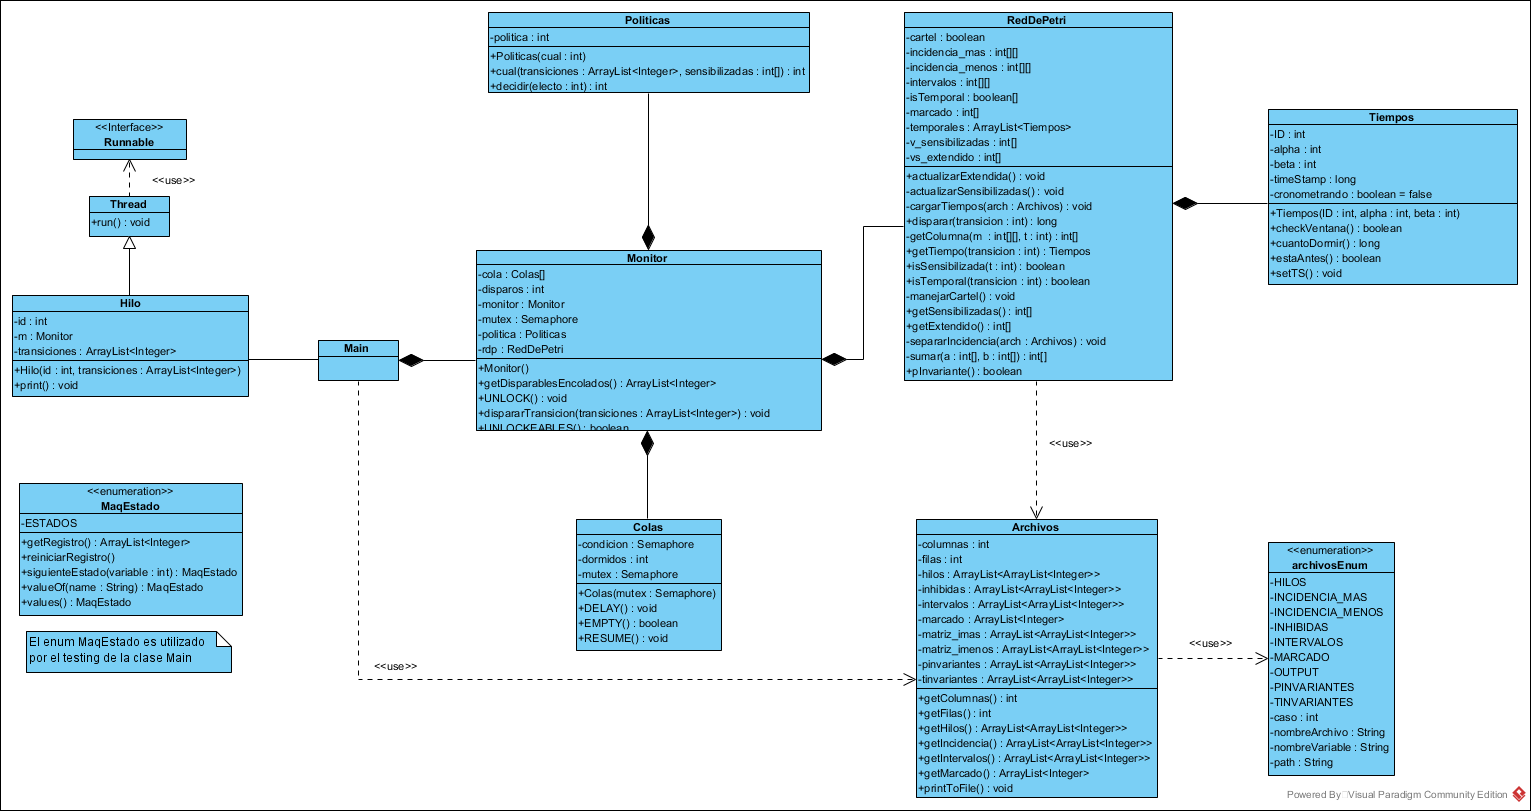
\includegraphics[width=15.5cm]{DClases.png}
    \label{fig:dclases}
    \caption{Diagrama de clases del sistema.}
\end{figure}

\subsection{Diagramas de secuencia}
\begin{figure}[H]
    \centering
    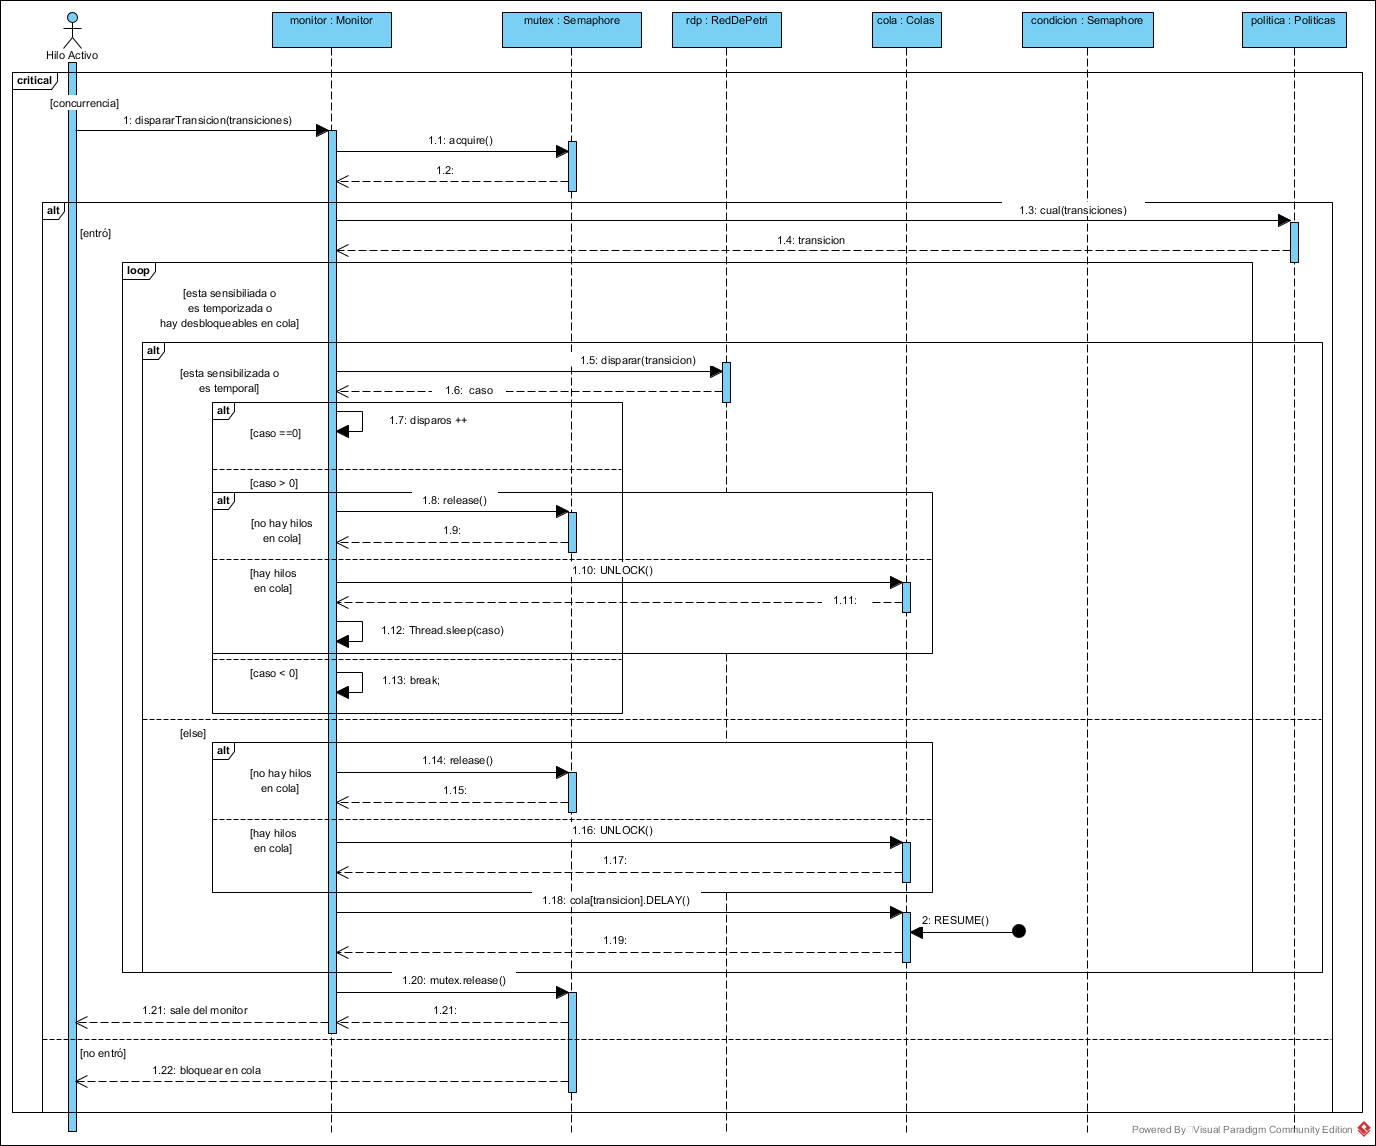
\includegraphics[width=15.5cm]{DSmonitor.png}
    \label{fig:dsmonitor}
    \caption{Diagrama del método `dispararTransicion' de la clase `Monitor'.}
\end{figure}

\begin{figure}[H]
    \centering
    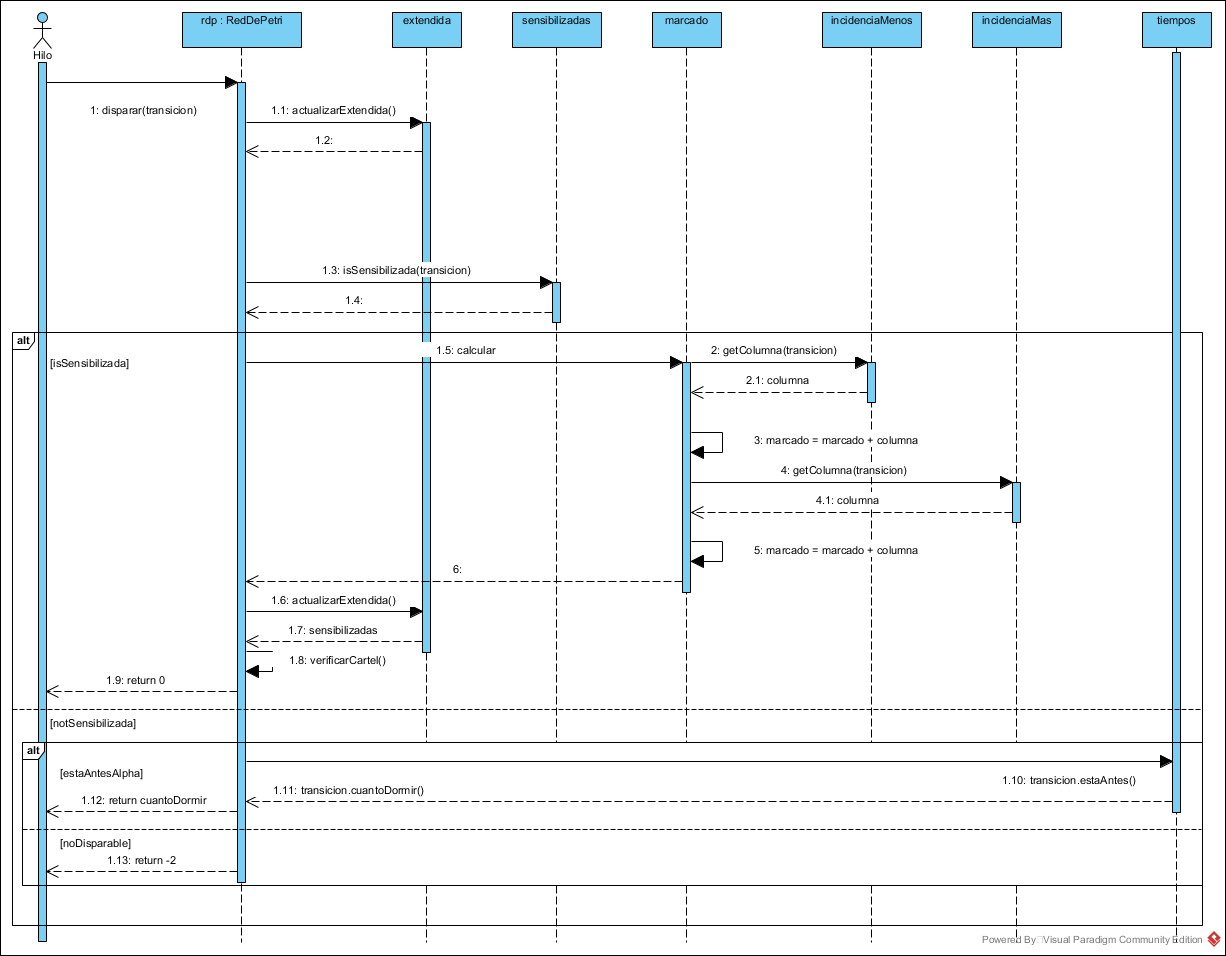
\includegraphics[width=15.5cm]{DSdisparo.png}
    \label{fig:dsdisparo}
    \caption{Diagrama del método `disparar' de la clase `RedDePetri'.}
\end{figure}

\section{Conclusiones y Resultados}
Se agregaron dos invariantes de transiciones más que el PIPE no las establecía, siendo éstos los invariantes correspondientes a la tercer entrada. Se cree que tiene una limitación en su cantidad de muestras, con esto mejoró significativamente la verificación de los disparos realizados.

Una vez realizados los \emph{testings}, se pudo verificar que ambos invariantes se cumplen, sin importar la cantidad de disparos realizados.

La cantidad  de ciclos completados tiene una relación de proporción directa con la magnitud de los disparos, por ejemplo, al realizar 5000 disparos, se completan 495 ciclos de T-Invariantes y con 10.000 disparos se completan 1022. Pero esto mismo no ocurre con los ciclos parciales, que por detenerse la ejecución, no alcanzaron a completarse.
Se observa que en ejecuciones que superan los 500 disparos aproximadamente, se comienza a establecer una constante de 60 ciclos sin completar, sin importar a cuanto se incremente la cantidad de disparos.

Como este valor de 60 coincide con la cota de la red, se podría sospechar que existe una interrelación entre ellos, de modo que una variación de dicha cota, también debería variar la cantidad de ciclos parciales. Se comprobó que esta hipótesis es válida, y variando la cota de la red influye directamente en la cantidad de ciclos sin completar, por lo que al reemplazar los 60 tokens que limitan la red, a 100 tokens, se obtuvieron exactamente 100 ciclos sin completar.

Como se mencionó en la \emph{sección 2.3}, el problema de interbloqueo de hilos que se produjo fue resultado de la mala implementación de la política y no de la distribución de hilos. Se probaron distintas distribuciones de hilos y todas resultaron en una ejecución exitosa.

El uso de una política u otra se aprecia claramente en los resultados. Al ejecutar 3000 disparos resultan las siguientes estadísticas:

\textbf{Política 1} -- Prioridad a T10 (planta baja) y salida indistinta.
\begin{itemize}[leftmargin=1.5cm]
    \item Disparos de T9: 101
    \item Disparos de T10: 197
    \item Disparos de T20: 119
    \item Disparos de T21: 120
\end{itemize}

\textbf{Política 2} -- Proridad a T21 (salida calle 2) y llenado indistinto.
\begin{itemize}[leftmargin=1.5cm]
    \item Disparos de T9: 104
    \item Disparos de T10: 191
    \item Disparos de T20: 71
    \item Disparos de T21: 165
\end{itemize}

La tendencia superior en T10 en la política 2 se debe a imprecisión del numero aleatorio generado por \textit{Math.random()} y a la consustancialidad de la red con ese numero de disparos.

\textbf{En síntesis, se puede concluir que se cumplieron todos los requerimientos funcionales del sistema propuestos, que la red evoluciona satisfactoriamente y que se respetan los principios teóricos de un monitor.}

\end{document}